% !TEX program = pdflatex
%
% 5-minute project presentation.
% Compile with: pdflatex main && pdflatex main
% Speaker notes are LaTeX comments throughout each frame.
%
\documentclass[aspectratio=169]{beamer}

\usetheme{metropolis}
\usepackage{graphicx}
\usepackage{booktabs}
\usepackage{xcolor}
\usepackage{tikz}
\usetikzlibrary{positioning, arrows.meta, shapes.geometric}

% ---------- accent palette (matches the report's figures) ----------
\definecolor{accent}{HTML}{08519c}      % deep blue (used for GRPO bar in Fig 1)
\definecolor{accentLight}{HTML}{6baed6} % light blue (SFT bar in Fig 1)
\definecolor{baselineGrey}{HTML}{bdbdbd}
\setbeamercolor{progress bar}{fg=accent}
\setbeamercolor{title separator}{fg=accent}
\setbeamercolor{normal text}{fg=black}
\setbeamercolor{alerted text}{fg=accent}

% Tighter frame title bar
\setbeamertemplate{frame numbering}[fraction]

% ---------- meta ----------
\title{Multi-turn GRPO with Real Tool Execution}
\subtitle{A null result on a 0.5B research agent}
\author{Yue Wu}
\date{April 2026}

\begin{document}

% ============================================================
% SLIDE 1 -- TITLE  (~20 s)
% ============================================================
\maketitle
% Speaker notes
% -------------
% Open with the one-line hook: "What happens when you train a small
% tool-using agent with REAL tool execution at every RL step? -- it
% turns out the answer is interesting, and not the one we expected."
%
% Don't dwell on the title slide. Move quickly.

% ============================================================
% SLIDE 2 -- PROBLEM / MOTIVATION  (~40 s)
% ============================================================
\begin{frame}{What is a research agent --- and what's the gap?}

\textbf{Research agent.} Language model that answers a question by
issuing real tool calls (search, read), reasoning over results,
over several rounds. ReAct, Toolformer, Perplexity, Deep Research.

\vspace{0.5em}

\textbf{The gap with current RL recipes.} DeepSeek-R1-style GRPO
trains on \emph{virtual} rollouts:
\begin{center}
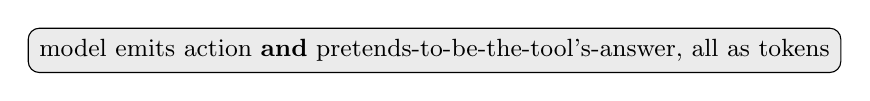
\begin{tikzpicture}[node distance=0.4em, font=\small]
\node[draw, rounded corners, fill=baselineGrey!30, inner sep=4pt]
  (v) {model emits action \textbf{and} pretends-to-be-the-tool's-answer, all as tokens};
\end{tikzpicture}
\end{center}
At inference the real retrieval index gives observations a 0.5B
policy would never hallucinate. \alert{Distribution mismatch.}

\vspace{0.5em}

\textbf{We close that gap.} Every GRPO rollout in training executes
the \emph{real} BM25 retrieval at every step, on a small open
0.5B-parameter policy.

% Speaker notes
% -------------
% "Research agents are the search-then-reason loop you see in
% Perplexity, ReAct, etc. Standard practice for training them with
% RL is to have the MODEL generate the tool output too -- it's
% cheaper, you don't need an external system. But that creates a
% distribution mismatch: at inference time the real retriever gives
% you observations that look NOTHING like what a 0.5B model would
% hallucinate. Our experiment is: what if we close that gap?
% Run real BM25 at every step during RL training, on a 0.5B model."
\end{frame}

% ============================================================
% SLIDE 3 -- METHOD  (~60 s, do not overrun)
% ============================================================
\begin{frame}{Method}

\textbf{Setup.} Qwen2.5-0.5B-Instruct + LoRA (rank~16, attention
\emph{and} MLP projections). HotpotQA distractor (2-hop QA), BM25
index over the 66k validation paragraphs.

\vspace{0.5em}

\textbf{Stage 1 --- SFT.} 6{,}000 synthetic 5-step traces
(\texttt{search} $\to$ \texttt{read} $\to$ \texttt{search} $\to$
\texttt{read} $\to$ \texttt{answer}) built from supporting facts
with \emph{real} retrieval. Loss masks out
\texttt{Observation:} tokens via the tokenizer's
\texttt{offset\_mapping} --- the policy is only scored on its own
JSON actions.

\vspace{0.5em}

\textbf{Stage 2 --- Multi-turn GRPO.} For each training question:
\begin{itemize}
  \item Sample $G{=}4$ rollouts; \alert{every \texttt{search}/\texttt{read} dispatched to the real BM25} between steps.
  \item Reward = correctness ($+1$) + format ($\le +0.10$) + efficiency ($-\alpha n_\mathrm{steps}-\beta n_\mathrm{lowJSD}$).
  \item Within-group $z$-score advantage $A_i = (R_i - \bar R)/\sigma_R$, no critic, no KL.
\end{itemize}

\vspace{0.3em}

\textbf{Engineering for T4 (16 GB).} Per-episode backward keeps
peak VRAM at one trajectory's activations.

% Speaker notes
% -------------
% "Two-stage. SFT on synthetic traces with REAL retrieval -- crucially
% we mask out the observation tokens from the loss, so the model is
% only trained to predict its own JSON actions, not to reconstruct
% the tool output. Then GRPO with real tool execution: G=4 rollouts
% per question, real BM25 between every step, within-group advantage,
% and -- importantly -- per-episode backward to fit on a T4."
%
% Don't read out the reward formula. Just say "combined reward of
% correctness, format, and efficiency."
\end{frame}

% ============================================================
% SLIDE 4 -- RESULT (THE REVEAL)  (~75 s, the most important slide)
% ============================================================
\begin{frame}{Result: 26\% $\to$ 44\% EM, but the decomposition is the story}

\begin{columns}[T, onlytextwidth]
\column{0.62\textwidth}
\centering
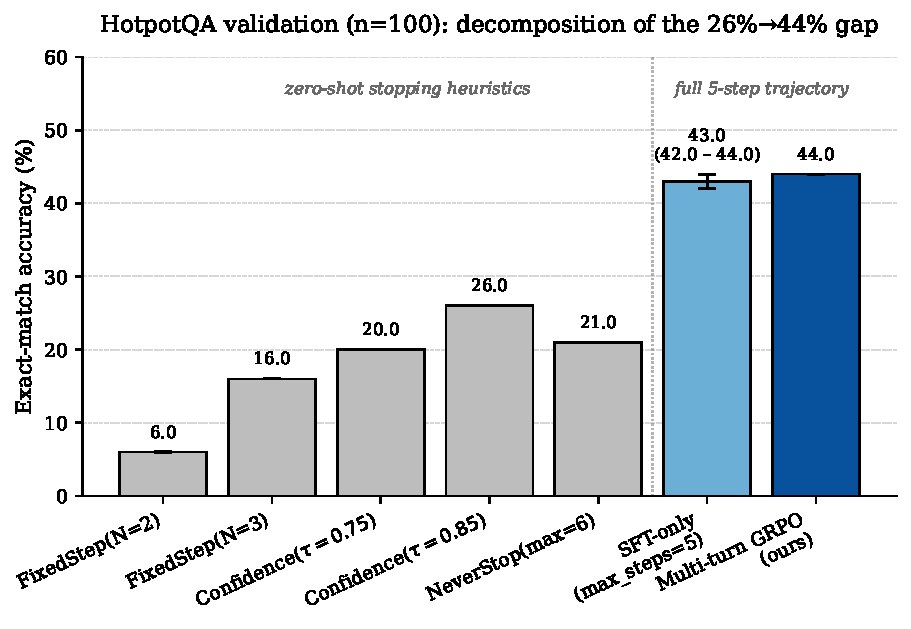
\includegraphics[width=\linewidth]{../report/figures/fig1_main.pdf}

\column{0.38\textwidth}
\textbf{Headline:} best zero-shot baseline 26\% $\to$ multi-turn GRPO 44\%, $+18$ EM.

\vspace{0.6em}

\textbf{But:} just letting the SFT model run for 5 steps (matching
the SFT trajectory length) gets \alert{42--44\%} \emph{with no RL}.

\vspace{0.6em}

\textbf{So:}\\
$\bullet$\, step-budget alignment $= +16$\\
$\bullet$\, GRPO on top $= 0$ within $\pm 5$ pp standard error.

\end{columns}

% Speaker notes
% -------------
% This is the slide that has to land. Slow down here.
%
% "Best zero-shot baseline is 26%, the GRPO model gets 44%. That's
% an 18-point lift -- looks like a clean win for RL." [pause]
%
% "But look at this row" -- point at SFT-only on the bar chart --
% "this is the SAME SFT model, no further training, just running for
% 5 steps instead of 2 or 3. It gets 42 to 44%."
%
% "Two independent runs of that same SFT model on the same 100
% questions gave 42 and 44 -- the GRPO number sits inside that
% within-run spread."
%
% "So the actual decomposition is: 16 of the 18 points come from a
% one-line inference-time change. GRPO contributes nothing within
% sampling error."
%
% Don't apologise. The audience just had their expectation flipped --
% pause for a beat to let it land before slide 5.
\end{frame}

% ============================================================
% SLIDE 5 -- DIAGNOSIS  (~55 s)
% ============================================================
\begin{frame}{Why GRPO didn't help: tied reward groups}

\textbf{Of 200 GRPO updates, only 41 were non-degenerate.}

\begin{center}

\begin{tikzpicture}[node distance=2.5em, font=\small]
\node[draw, rounded corners, fill=baselineGrey!30, minimum width=4cm, minimum height=1.2cm]
  (nominal) {200 nominal updates};
\node[draw, rounded corners, fill=accent, text=white, minimum width=4cm, minimum height=1.2cm, right=3em of nominal]
  (effective) {\textbf{41 effective updates}};
\draw[-{Stealth}, thick, accent] (nominal) -- node[above, text=black] {\footnotesize 159 tied groups skipped} (effective);
\end{tikzpicture}
\end{center}

\textbf{The mechanism.} The format reward saturates at $+0.10$ as
soon as the policy emits valid JSON with the required keys.
Within a group of $G{=}4$ all-wrong rollouts:
\begin{itemize}
  \item correctness tied at 0,
  \item format tied at 0.10 (every rollout is well-formed),
  \item efficiency tied at $-\alpha\cdot 5$ (every rollout uses 5 steps).
\end{itemize}
Tied rewards $\Rightarrow$ within-group advantage $A_i \to 0$
$\Rightarrow$ \alert{no gradient}. The skip-on-tied guard fires on 80\% of training questions.

% Speaker notes
% -------------
% "The mechanism is simple. The within-group advantage formula
% subtracts the group mean and divides by the group std. If all 4
% rollouts get the same reward, advantage is zero, no gradient.
% That happens when the format reward saturates, which it does
% almost immediately because our SFT model already emits valid JSON.
% So on every all-wrong group of rollouts -- which is 80% of training
% questions -- there's nothing for GRPO to push on. The 200 updates
% are really 41."
\end{frame}

% ============================================================
% SLIDE 6 -- LIMITATIONS + NEXT STEP  (~35 s)
% ============================================================
\begin{frame}{Limitations and what we'd do next}

\textbf{Limitations of this evaluation.}
\begin{itemize}
  \item $n{=}100$ HotpotQA val: Wald SE $\approx \pm 5$~pp, can't resolve sub-2-pp gaps.
  \item No KL-to-reference term --- T4-memory driven, not principled.
  \item 0.5B scale: format-saturation mechanism likely changes at 7B+.
\end{itemize}

\vspace{0.6em}

\textbf{The concrete next step is reward design, not more compute.}

A format-reward term with \emph{continuous intra-group variance}
(token-level JSON-validity score, query-novelty score from lexical
overlap with previous queries, doc-overlap score across rollouts)
would give a usable gradient on the 80\% of currently-tied
training groups. We expect this to move the needle more than
running GRPO longer.

% Speaker notes
% -------------
% "Three honest limitations -- 100 questions is a small eval, the
% KL term we omitted was a memory call not a principled one, and
% 0.5B is small enough that things change at scale. But the
% prescription is clear: don't run GRPO longer; fix the reward
% so it actually has variance to push on. Continuous-variance
% format terms are the obvious thing."
\end{frame}

% ============================================================
% SLIDE 7 -- CLOSING  (~15 s)
% ============================================================
\begin{frame}[standout]
Match training and inference \emph{trajectory length} first.

\vspace{0.7em}

Then fix the saturating reward, before reaching for more RL.

\vspace{1.2em}

{\small Paper, code, and tuning post-mortem:\\
\texttt{github.com/202520030411/Research\_Agent\_RL}}

% Speaker notes
% -------------
% "One sentence to take away: match training and inference trajectory
% length first; THEN fix the saturating reward -- before reaching for
% more RL. Code and the full paper are in the repo. Happy to take
% questions."
\end{frame}

% ============================================================
% BACKUP SLIDES (do not show unless asked)
% ============================================================
\appendix

\begin{frame}{Backup: stop-reason breakdown across baselines}
\centering\small
\begin{tabular}{lrrr}
\toprule
Method & \texttt{answer} & \texttt{parse\_error} & \texttt{policy} \\
\midrule
FixedStep($N{=}2$)         & 0  & 0   & 100 \\
FixedStep($N{=}3$)         & 0  & 50  & 50  \\
Confidence($\tau{=}0.75$)  & 7  & 48  & 45  \\
Confidence($\tau{=}0.85$)  & 12 & 44  & 44  \\
NeverStop($\max{=}6$)      & 53 & 47  & 0   \\
\bottomrule
\end{tabular}

\vspace{0.7em}

The \texttt{answer} column is the rate at which the SFT policy
emits a clean \texttt{action:"answer"} step. At
$\mathrm{max\_steps}\leq 3$, this rate is 0--12\%; at the full
5-step budget (matching SFT) it would saturate the EM.
\end{frame}

\begin{frame}{Backup: why no KL-to-reference term}
\textbf{Memory-driven, not principled.}

\begin{itemize}
  \item Our per-episode-backward trick caps peak VRAM at \emph{one}
  trajectory's activations ($\approx 6$--$8$~GB at 1{,}500 tokens
  bf16, T4 16~GB).
  \item KL term needs a second forward through a frozen reference
  policy on the same trajectory, doubling activation memory.
  \item PEFT \texttt{disable\_adapter} saves \emph{weights} memory
  but the second set of \emph{activations} still has to be resident
  before \texttt{loss.backward()}.
  \item LoRA's $\sim$2 M trainable params already act as a capacity
  regulariser for a 200-step run.
  \item Re-introduce the KL term at larger adapters / longer runs / bigger GPUs.
\end{itemize}
\end{frame}

\begin{frame}{Backup: three failure modes during tuning}
\small
\begin{enumerate}
  \item \textbf{Rollout temperature 0.9} (DeepSeek-R1 default) breaks
  JSON format on the 0.5B policy --- every rollout dies at step 1.
  Fix: $T{=}0.5$.
  \item \textbf{$\mathrm{max\_steps}{=}3$} cuts the 2-hop trajectory
  in half. Rollout pattern is
  \texttt{search}$\to$\texttt{read}$\to$\texttt{search} --- never
  reaches \texttt{answer}. Fix: $\mathrm{max\_steps}{=}5$, matching
  SFT.
  \item \textbf{\texttt{torch.no\_grad()} disables gradients but not
  dropout.} LoRA dropout active during rollout corrupts generations.
  Symptom: \texttt{steps=1.0, loss=0.0} during training while
  \texttt{[VAL]} reports $\sim$35\% (eval-mode). Fix:
  \texttt{model.eval()} before rollout, \texttt{model.train()}
  after.
\end{enumerate}

\vspace{0.5em}

Common thread: each was a default that worked for a larger base
policy or a non-interactive loop, and was silently wrong here.
\end{frame}

\begin{frame}{Backup: full results table}
\centering
\small
\begin{tabular}{lcc}
\toprule
Method & EM (\%) & Avg.\ steps \\
\midrule
FixedStep($N{=}2$)        & 6.0  & 2.00 \\
FixedStep($N{=}3$)        & 16.0 & 2.50 \\
Confidence($\tau{=}0.75$) & 20.0 & 2.88 \\
Confidence($\tau{=}0.85$) & 26.0 & 3.20 \\
NeverStop($\max{=}6$)     & 21.0 & 3.57 \\
\midrule
\textbf{SFT-only @ $\max_{\text{steps}}{=}5$}$^{\dagger}$ & \textbf{42.0\,/\,44.0} & \textbf{5.00} \\
\textbf{Multi-turn GRPO (ours)}                         & \textbf{44.0}          & \textbf{4.99} \\
\bottomrule
\end{tabular}

\vspace{0.5em}
{\footnotesize $^{\dagger}$ Two independent evaluations of the same
SFT adapter on the same 100 questions at $T{=}0.1$. The 2-pp
spread is the within-run sampling variance at $n{=}100$; GRPO
sits inside that spread.}
\end{frame}

\end{document}
